\chapter{AI-FML人機共學}
% ch1-1
\section{什麼是AI人工智慧}
\subsection{什麼是AI人工智慧}
 人工智慧(Artificial Intelligence)是指通過計算機系統模擬人類智能的能力。它涉及機器學習、自然語言處理、計算機視覺等技術,旨在讓機器能夠學習、推理、解決問題,並進行決策。
\subsubsection{人類智慧和人工智慧的差異}
\begin{itemize}
    \item 學習方式:\\
        人類智慧:通過經驗、情感和社會互動學習,具有靈活性和創造性。\\
        人工智慧:通常依賴大量數據和算法進行學習,專注於特定任務,並且在某些情況下比人類更高效。
    \item 情感與意識: \\
        人類智慧:擁有情感、直覺和意識,能夠理解和感受複雜的情感和社會關係。\\
        人工智慧:缺乏真正的情感和意識,只能根據預定的規則和數據做出反應。
    \item 推理能力: \\
        人類智慧:能夠進行抽象思考和道德判斷,能夠在不確定性中做出決策。\\
        人工智慧:通常依賴於具體的數據和模式,可能在面對新情境時表現不佳。 
\item 適應能力:\\
        人類智慧:具有高度的適應性,能夠靈活應對不同的情境和挑戰。\\
        人工智慧:在特定任務上表現出色,但在新情境或未見過的情況下,適應性較差。
\end{itemize}

\subsubsection{機器人有左右腦嗎?}
機器人和人工智慧的運作基於算法和數據處理,並不具備生物學上的左右腦結構。它們的“思考”是通過程式碼、數據模型和計算過程來實現的。因此,雖然機器可以模擬某些認知功能,但並沒有類似人類大腦的分區和功能劃分。 \newpage

\subsubsection{人類可以幫助機器人建置他們的大腦嗎?}
人類可以幫助機器人建置和改進它們的「大腦」,這通常是指它們的人工智慧系統。以下是幾種方式:
\begin{itemize}
    \item 數據訓練:人類可以提供大量的數據來訓練機器學習模型,這些數據可以幫助機器人理解和學習特定任務。
    \item 算法設計:工程師和研究人員可以設計新的算法,提升機器人的推理、學習和決策能力。 
    \item 調整和優化:通過不斷的測試和反饋,人類可以優化機器人的行為,使其在特定環境中表現更好。 
    \item 倫理和規範:人類在建置機器人系統時,還需要考慮倫理和法律問題,以確保技術的安全和合乎道德。
\end{itemize}

\subsubsection{人類可以幫助機器人建置他們的左右腦嗎?}
可以在機器人的人工智慧系統中模擬類似於人類左腦和右腦的功能,但這不是通過物理結構實現的,而是通過軟體架構和算法設計。
\begin{itemize}
    \item 模塊化設計:可以開發專門的模塊,分別負責不同的功能。例如,一個模塊可以專注於邏輯推理和數據分析(類似於左腦),而另一個模塊可以處理創造性任務和直覺判斷(類似於右腦)。
    \item 多樣化算法:使用不同類型的算法來模擬不同的思考方式。例如,使用機器學習算法進行模式識別(類似於直覺),同時使用規則基礎的系統來處理邏輯問題。
    \item 整合系統:透過系統整合,將這些模塊和算法結合在一起,使機器人能夠在不同的情境中靈活切換。
\end{itemize}

\subsection{科學家認為人工智慧有哪些特性?}
\begin{enumerate}
    \item 自學能力:能從數據中學習和改進,而不是僅依賴預先編程的規則。
    \item 適應性:能根據新的環境或數據變化調整其行為和決策。
    \item 推理能力:能根據已知信息推斷出新的結論或解決問題。
    \item 模式識別:能識別數據中的模式和趨勢,這對於圖像識別和語音識別特別重要。
    \item 自然語言理解:能理解和生成自然語言,便於與人類進行交流。
    \item 多任務處理:能同時處理多個任務,並在不同任務之間切換。
    \item 預測能力:基於過去的數據進行預測,幫助做出未來的決策。
    \item 自主性:在某些情況下,能獨立做出決策,而不需人類的干預。
\end{enumerate}
\subsubsection{什麼是圖靈測試以及模仿遊戲電影}
圖靈測試是由英國數學家艾倫·麥席森·圖靈(Alan Mathison Turing)提出的,用於評估機器是否具備人類水平的智能。在測試中,一個評判者與一個人類和一個機器進行對話。如果評判者無法可靠地分辨出哪一個是人類,則該機器被認為通過了測試。\\
\par《模仿遊戲》是一部2014年的電影,講述了阿蘭·圖靈的故事,他在二戰期間破解了德國密碼,並探討了他的生平、工作以及對AI的早期思考。電影突顯了他在數學和計算機科學上的貢獻,也涉及他面對的社會和個人挑戰。
\subsubsection{知識本體論(Ontology)}
知識本體論(Ontology)是哲學的一個分支,研究存在的本質和類別。它涉及到如何分類和理解不同類型的實體及其關係。在AI的背景下,這種思考可以幫助理解機器如何組織和處理知識。
\subsubsection{AI可以模仿人類的思考和活動嗎?}
AI能夠模擬人類部分的理性思考與人性化行為
\begin{itemize}
    \item 人性化思考:\\
        AI可以模擬某些人性化的思考過程,例如通過自然語言處理來進行對話,但並不具備真正的情感或意識。
    \item 理性化思考:\\
         AI能夠使用邏輯和算法進行分析和推理,模仿人類的理性思考,但其過程仍然是基於數據和預先設定的規則。
    \item 人性化活動:\\
        AI可以模擬一些人性化的活動,例如社交互動或藝術創作,但這些行為並不基於人類的情感或經驗,而是根據算法和數據。
    \item 理性化行動:\\
        AI可以模擬理性行動,通過計算最佳路徑或選擇來解決問題,這通常涉及決策支持系統和優化算法。
\end{itemize}
\newpage

\subsection{AI人工智慧知識圖}
使用以上的內容做為文本並分別使用TAIDE, Zephyr, Llama 3模型產生知識圖。
\knowledgeGraph{images/w3/w3_taide.png}{什麼是人工智慧-TAIDE}{fig:w3-TAIDE}{8}{\item 知識圖複雜且多樣化,顯示了廣泛的關聯性,節點之間的連接清晰可見}{\item 缺乏明確的層次結構或中心主題}{0.3}

\knowledgeGraph{images/w3/w3_zephyr.png}{什麼是人工智慧-Zephyr}{fig:w3-Zephyr}{8}{\item 清晰的視覺層次,有明確的中心節點和子節點
\item 使用不同的顏色和大小來區分節點的重要性
}{\item 部分區域節點過於集中,可能造成重疊
}{0.3}

\knowledgeGraph{images/w3/w3_llama3.png}{什麼是人工智慧-Llama3}{fig:w3-Llama3}{7}{\item 整體結構清晰,分組明確
}{\item 存在一個過大且信息量低的"沒有"節點,佔據了圖的重要位置
\item 可能表明模型在某些領域的知識或理解存在明顯缺陷。
}{0.3}


% 第七周的臺南大學AI機器人新聞報導(今周刊)
\section{臺南大學AI機器人新聞知識圖}
根據今周刊對臺南大學李健興教授與團隊運用機器人幫助小朋友學臺語的報導 \cite{ref:AIRobot-taiwanese}產生知識圖。

\knowledgeGraph{images/w7/AIRobot-taide.png}{今周刊報導-TAIDE}{fig:w7-taide}{8.5}{\item 完整捕捉到教育相關概念(教師、學生、教導和學習)
}{\item 台語相關內容呈現不夠突出}{0.2}

\knowledgeGraph{images/w7/AIRobot-Zephyr.png}{今周刊報導-Zephyr}{fig:w7-zephyr}{7}{\item 多語言支援(英語、日語)表現清晰
\item 結構相對簡潔
}{\item 本土特色(如諧音梗理解)未能體現}{0.3}


\knowledgeGraph{images/w7/AIRobot-Llama3.png}{今周刊報導-Llama3.2}{fig:w7-llama3}{7.5}{\item 突出展示了多方主體(教師、學生、公司)
\item 節點之間的連接較為緊密
}{\item 重要概念(如本土訓練、教育解放)未能清楚呈現}{0.3}



% week 8 台英慧虛擬機器人體驗結合科技大觀園報導

% 台英慧

\section{台英慧虛擬AI機器人輔助學習}
台英慧是由國立台南大學李健興教授及其研究團隊,聯合國家高速網路與計算中心、真平語文企業、女媧創造機器人及優必達公司,推出的虛擬機器人。
\subsection{實體機器人沒有的優勢}
先前國立臺南大學李建興教授和其研究團隊設計了「TAIDE 臺英語機器人」幫助國小學童學習台語以及英語。TAIDE台英語機器人支援多模態輸入,包括聲音、影像和文字,能夠說普通話,台語,日語以及英文,也能夠顯示圖片和產生知識圖。\par
但是它的缺點也很明顯,必須要有實體機器人才能實際操作,這增加了推廣的難度,而「台英慧虛擬聊天機器人」就彌補了這項缺陷,使用者只需要網路就能夠使用虛擬機器人進行輔助學習,相對於實體機器人來說,台英慧也有更高的靈活性,他的虛擬形象有各式的動作能夠提高互動性,而且它也能夠使用深度學習與自然語言處理技術,生成台語教學所需的圖片資源,幫助學生透過互動式學習提高語言學習效率。


\subsection{台英慧實際操作體驗}
這次課程中我體驗了台英慧的一般對話功能以及它的圖片生成功能。

\subsubsection{一般對話功能}
由於學校電腦沒有麥克風,所以我使用文字輸入的方式和台英慧進行對話。我問了他可不可以推薦我要吃什麼早餐,它回答了一個早餐食譜作為關鍵字的Google網址。後來我告訴他我想要吃中式早餐,它給我一個中式早餐食譜作為搜索關鍵字的網址。
\begin{figure}[htbp!]
    \centering
    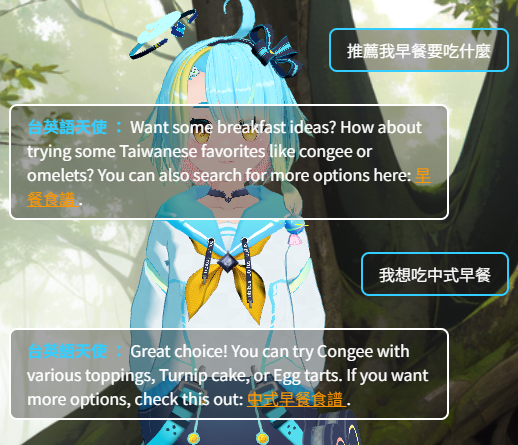
\includegraphics[width=0.5\linewidth]{images/w8/AIhist.png}
    \caption{台英慧對話紀錄}
    \label{fig:w8-chat-history}
\end{figure}


\subsubsection{圖片生成}
接著我使用了它的圖片生成功能,台英慧會根據使用者的輸入訊息將它的背景圖片進行更換。第一次我輸入的提示詞為\textbf{畫一棵大樹},結果如\autoref{fig:w8-taiyinghui-tree}。第二次輸入為\textbf{生成飛機},結果為\autoref{fig:w8-taiyinghui-airplane}。

\begin{figure}[htbp!]
	\centering
	% 圖片一(左)
	\begin{minipage}{0.4\linewidth}
		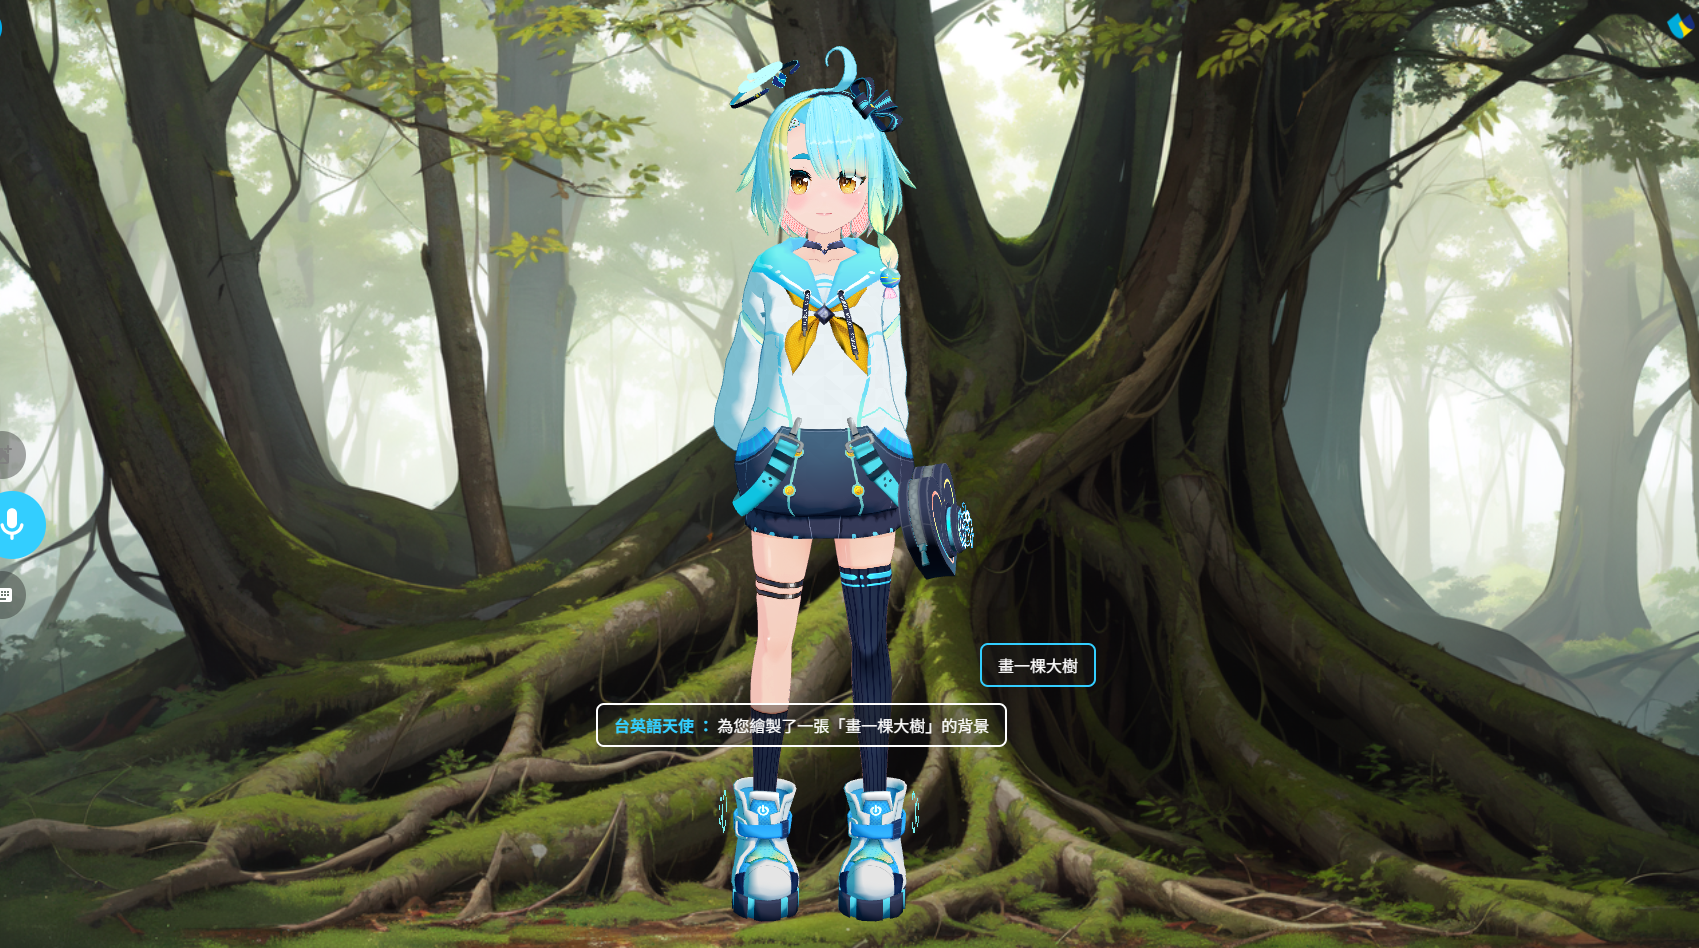
\includegraphics[width=\linewidth]{images/w8/AIdraw.png}
		\caption{台英慧生成大樹}
        \label{fig:w8-taiyinghui-tree}
	\end{minipage}
    \hspace{2em}
	% 圖片二(右)
	\begin{minipage}{0.4\linewidth}
		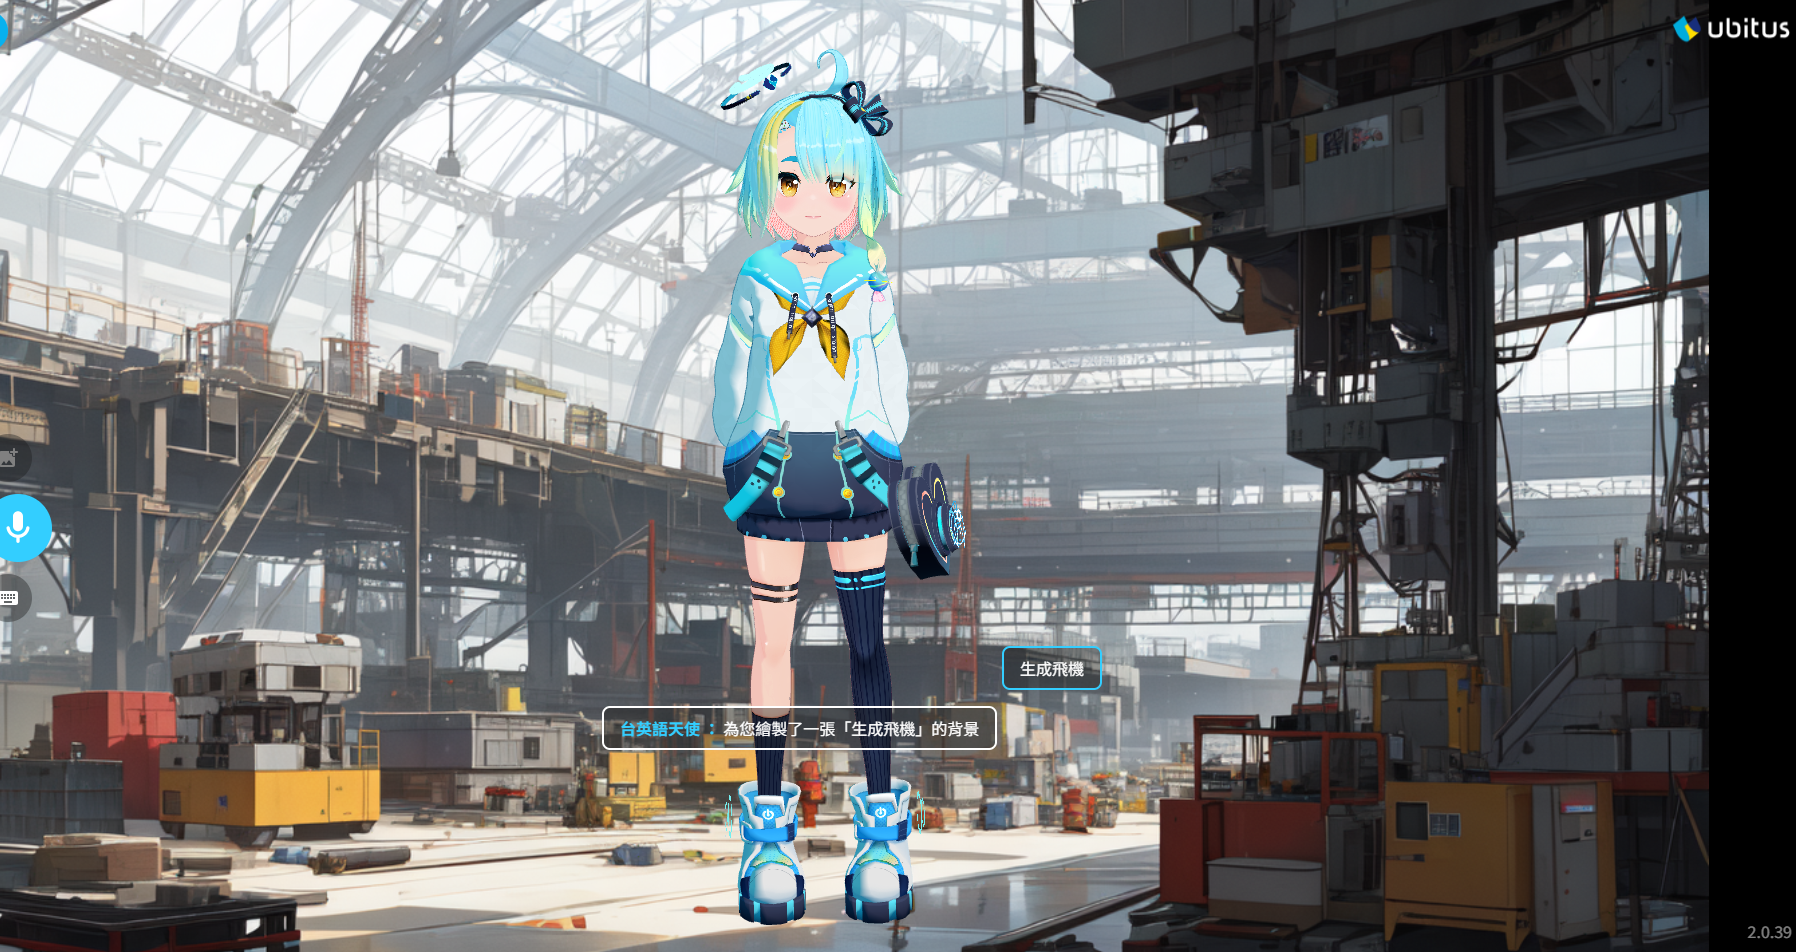
\includegraphics[width=\linewidth]{images/w8/AI飛機.png}
		\caption{台英慧生成飛機}
        \label{fig:w8-taiyinghui-airplane}
	\end{minipage}
\end{figure}



\subsubsection{初次體驗評分及心得}
\begin{itemize}
    \item 一般對話(7/10): 比較希望能夠給我實際的推薦名單,而不是給我搜索網址讓我自己找。
    \item 圖片生成(8/10): 大樹的照片有符合而且看起來還不錯,但是飛機變成工廠了。
    \item 心得: 這次的體驗讓我看到了很多台英慧的優點以及缺點,它的語音識別能力不錯,能夠識別台語。除此之外它也有一些特殊的動作和表情,例如跳舞。但比較遺憾的是目前它只會說英語,還沒辦法說台語或普通話,而且在\autoref{fig:w8-taiyinghui-airplane}中,它好像把我的提示詞理解為生成飛機的地方而不是飛機本身,所以圖片結果是工廠。
\end{itemize}

\subsection{台英慧對話知識圖}
\textRightGraphLeft{images/w8/taiyinghui-taide}{台英慧-TAIDE}{taiyinghui-taide}{8}{能夠根據對話內容,很好地概括和表達早餐的相關知識}{有一個\textbf{子}和\textbf{沒有}節點}{0.4}

\textRightGraphLeft{images/w8/taiyinghui-zephyr}{台英慧-Zephyr}{taiyinghui-zephyr}{7}{有抓到中式早餐這個重點}{沒有太多具體的早餐選項}{0.4}

\textRightGraphLeft{images/w8/taiyinghui-llama3}{台英慧-Llama 3.2}{taiyinghui-llama3}{6}{知識圖能夠反映對話內容的主要主題和概念}{知識圖的結構較為鬆散,節點和邊之間的聯繫不夠緊密}{0.4}

\section{大型語言模型參數數量比較}
這次上課我分別和Llama 3.1 TAIDE 8B(\autoref{fig:8B})以及Llama 3.1 70B(\autoref{fig:70B})的模型進行比較,並且對比了他們的回答。\\


\begin{figure}[htbp!]
	\centering
	% 圖片一(左)
	\begin{minipage}{0.4\linewidth}
        \vspace{1.2em}
		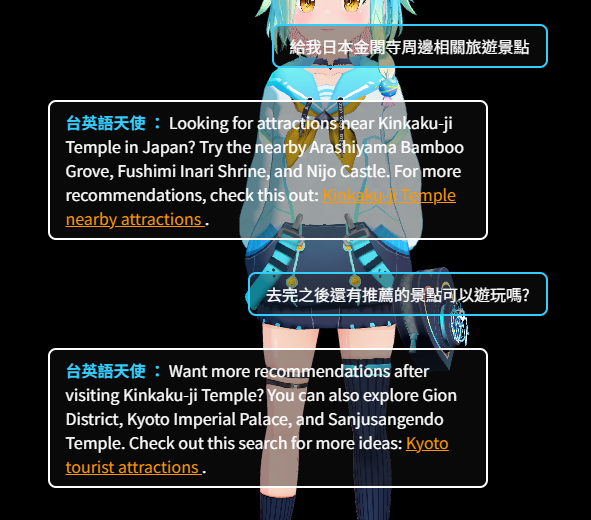
\includegraphics[width=\linewidth]{images/w9/8B.png}
		\caption{8B參數模型回答}
        \label{fig:8B}
	\end{minipage}
    \hspace{1em}
	% 圖片二(右)
	\begin{minipage}{0.4\linewidth}
		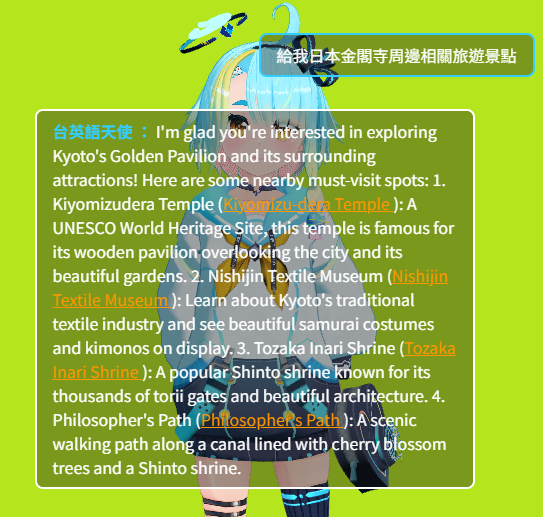
\includegraphics[width=\linewidth]{images/w9/70B.png}
		\caption{70B參數模型回答}
        \label{fig:70B}
	\end{minipage}
\end{figure}
在比較兩個模型的回答風格後,8B模型的回應較為簡潔,偏向於快速滿足提問,給出直接的景點名稱並附上超連結,讓使用者自行點擊查看更多資訊。然而,這種方式雖然有效率,但少了一些豐富的內容,使得整體回答較為單薄。相比之下,70B模型的回應則顯得細膩得多,除了介紹景點名稱,還加上了景點的歷史背景、特色和吸引力。這讓使用者在不點擊連結的情況下,便能深入了解各景點的獨特之處,讓回答更具畫面感和情境。

\subsection{知識圖比較}

\textRightGraphLeft{images/w9/llama3-8B}{8B參數模型}{fig:Llama3-8B}{6}{簡單易讀、直觀清晰}{連結信息有限、缺乏細節}{0.5}
\textRightGraphLeft{images/w9/llama3-70B}{70B參數模型}{fig:Llama3-70B}{9}{多層次連結、結構完整,易於辨認且有助於旅遊規劃}{視覺複雜,不好看出主要信息}{0.5}

使用Llama 3.2對兩個不同參數的模型進知識圖生成,可以看到70B參數模型(\autoref{fig:Llama3-70B})的知識圖比8B(\autoref{fig:Llama3-8B})參數模型更加詳細,有更多的連結和細節,但也因此顯得較為複雜。而8B參數模型的知識圖則相對簡單易讀,8B 知識圖適合想要快速查詢京都主要景點的使用者。其簡單的結構讓人可以快速理解,但缺乏深度和多樣性,適合短期或粗略的旅行規劃。70B 知識圖適合想要深入探索京都文化、活動和小眾景點的旅客。兩個不同參數的模型各有優缺點,使用者可以根據自己的需求選擇適合的模型。

